\documentclass[10pt,twocolumn,letterpaper]{article}

\usepackage{cvpr}
\usepackage{times}
\usepackage{epsfig}
\usepackage{graphicx}
\usepackage{amsmath}
\usepackage{amssymb}
\usepackage[utf8x]{inputenc}
\renewcommand{\refname}{Bibliografia}
\usepackage{listings}
\renewcommand{\lstlistingname}{}
\renewcommand{\figurename}{Figura}


\usepackage{url}

% Include other packages here, before hyperref.

% If you comment hyperref and then uncomment it, you should delete
% egpaper.aux before re-running latex.  (Or just hit 'q' on the first latex
% run, let it finish, and you should be clear).
%\usepackage[pagebackref=true,breaklinks=true,letterpaper=true,colorlinks,bookmarks=false]{hyperref}

\cvprfinalcopy % *** Uncomment this line for the final submission

\def\cvprPaperID{****} % *** Enter the CVPR Paper ID here
\def\httilde{\mbox{\tt\raisebox{-.5ex}{\symbol{126}}}}

% Pages are numbered in submission mode, and unnumbered in camera-ready
\ifcvprfinal\pagestyle{empty}\fi
\begin{document}

%%%%%%%%% TITLE
\title{Parallel Computing Final\\BigramTrigramGenerator con Java, Java Threads \& C++ Threads}

\maketitle
\thispagestyle{empty}

%%%%%%%%% ABSTRACT
\begin{abstract}
L'obiettivo di questo progetto è quello di calcolare le occorrenze dei bigrammi e trigrammi di lettere con tre approcci diversi: uno sequenziale (in Java) e due paralleli (rispettivamente con Java Thread e C++ Thread). I risultati vengono espressi in termini di tempo computazionale complessivo e Speedup.
\end{abstract}

%%%%%%%%% BODY TEXT
\section{Introduzione}
L'algoritmo, che viene utilizzato per la ricerca di bigrammi e trigrammi di lettere all'interno di un testo di lunghezza variabile, si presta bene alla parallelizzazione in quanto due o più thread possono lavorare nello stesso momento su porzioni di testo differenti.
   
\subsection{Bigrammi \& Trigrammi}
In generale un \textit{n-gramma} è una sottosequenza di n elementi di una data sequenza, gli elementi in questione possono essere sillabe, lettere, parole, ecc.\cite{N-GRAMMA}\newline
Per questo progetto ci siamo occupati di n-grammi di lettere. In particolare:
\begin{itemize}
	\item Una sequenza di due lettere si dice \textit{Bigramma} o \textit{Digramma}
	\item Una sequenza di tre lettere si dice \textit{Trigramma}
\end{itemize}

\subsection{Descrizione del Dataset}
Il dataset utilizzato è stato estratto dal database del \textit{Progetto Gutenberg}, una biblioteca digitale di eBook di pubblico dominio, liberamente riproducibili e scaricabili \cite{GUTENBERG}. Il testo scelto è \textit{"La scienza in cucina e l'arte di mangiar bene"} di Pellegrino Artusi \cite{ARTUSI}. Per eseguire gli esperimenti il testo è stato accorciato e allungato in modo da ottenere file di dimensioni diverse: 50kb, 100kb, 200kb, 500kb, 1mb, 2mb, 4mb, 8mb, 16mb, 32mb.

\subsection{Specifiche Hardware}
Per questi esperimenti è stato utilizzato un MacBook Pro (Retina, 13-inch, Mid 2014) con le seguenti specifiche:
\begin{itemize}
	\item Processore 2,6 GHz Dual-Core Intel Core i5
	\item Memoria 8 GB 1600 MHz DDR3
	\item Memoria Flash Storage 128 GB
\end{itemize}

\section{Implementazione}
Sono state eseguite tre implementazioni, una in maniera sequenziale in linguaggio Java e due in maniera parallela rispettivamente con Java Thread e C++ Thread.

\subsection{Versione Sequenziale in Java}
La versione sequenziale dell'algoritmo è piuttosto semplice. È stata utilizzata una classe \textit{"LinesExtractor"} che prende in input il nome del file txt ed espone un metodo \textit{extractLines} che restituisce una lista di tutte le righe del testo escludendo per semplicità righe vuote e caratteri speciali. L'estrazione delle righe avviene tramite la funzione \textit{readAllLines} della classe \textit{"Files"} standard del Java. 
\begin{lstlisting}[basicstyle=\scriptsize, language=Java, frame=single, caption={Esempio di estrazione di righe da un file in Java},captionpos=b, showstringspaces=false, mathescape=true]
public List<String> extractLines() {
  List<String> finalLines = new ArrayList<>();
  List<String> lines = null;
  String regex = "[$\hat{}$A-Za-z0-9' ]";

  try {
    FileSystem fs = FileSystems.getDefault();
    lines = Files.readAllLines(fs.getPath("", filename));
  } catch (IOException e) {
    System.out.println("Failed to read " + filename);
  }
  lines.forEach(line -> {
    if (!line.isBlank() && !line.isEmpty()) {
      line = line.toLowerCase().replaceAll(regex, "");
      finalLines.add(line);
    }
  });
  return finalLines;
}  
\end{lstlisting}

La funzione principale prende in input questa lista di righe ed estrae la lista di tutte parole al suo interno tramite un'espressione regolare (\textit{\textbackslash \textbackslash s+}). 
\begin{lstlisting}[basicstyle=\scriptsize, language=Java, frame=single, caption={Esempio di estrazione di parole},captionpos=b, showstringspaces=false]
LinesExtractor extractor = new LinesExtractor(filename);
List<String> lines = extractor.extractLines();

List<String> words = new ArrayList<>();
lines.forEach(line -> {
  words.addAll(Arrays.asList(line.split("\\s+")));
});

words.removeAll(Collections.singleton(""));
\end{lstlisting}

A questo punto vengono calcolati i bigrammi o i trigrammi per ognuna delle parole estratte. \newline
Il tempo di esecuzione viene misurato con la funzione \textit{currentTimeMillis()} della libreria standard \textit{System}.
\begin{lstlisting}[basicstyle=\scriptsize, language=Java, frame=single, caption={Esempio di ricerca di bigrammi/trigrammi},captionpos=b, showstringspaces=false]
long start = System.currentTimeMillis();

int n = 2; // 2: bigrammi, 3: trigrammi

List<String> ngrams = new ArrayList<>();
for (String word: words) {
  if (word.length() >= n) {
    for (int i = 0; i < word.length() - (n - 1); i++) {
      ngrams.add(word.substring(i, i + n));
    }
  }
}

long end = System.currentTimeMillis();
\end{lstlisting}

\subsection{Versione Parallela con Java Thread}
Per la versione parallela con Java Thread, la classe \textit{"LinesExtractor"} è la stessa della versione sequenziale ed è uguale anche la metodologia con cui vengono estratte le parole.\newline
Per il conteggio dei bigrammi o trigrammi è stato utilizzato un \textit{AtomicInteger} in modo che ogni thread possa aggiornarlo evitando inconsistenze.\newline
È stata creata una classe \textit{NGramThread} che estende la classe \textit{Thread} e il suo costruttore prende in ingresso:
\begin{itemize}
	\item \textit{globalCounter}: riferimento alla variabile \textit{AtomicInteger}
	\item \textit{words}: l'intera lista di parole
	\item \textit{n}: intero che specifica se vengono trattati bigrammi (\textit{n==2}) oppure trigrammi (\textit{n}==3)
	\item \textit{start} e \textit{stop}: due interi che indicano gli indici di partenza e arrivo del range di parole su cui il thread lavora
\end{itemize}

La classe presenta anche un intero \textit{nGramCounter} inizializzato a zero e che viene incrementato ad ogni n-gramma trovato. Una volta calcolato tutti gli n-grammi si aggiorna il valore dell'intero atomico \textit{globalCounter} tramite la funzione \textit{addAndGet} della classe \textit{"AtomicInteger"} nel package \textit{"java.util.concurrent.Atomic"}, aggiungendo in maniera atomica il valore di \textit{nGramCounter}.

\begin{lstlisting}[basicstyle=\scriptsize, language=Java, frame=single, caption={Esempio di ricerca di bigrammi/trigrammi con Java Thread},captionpos=b]
public class NGramThread extends Thread {

  private int n, start, stop;
  private List<String> words;
  private AtomicInteger globalCounter;
  private int nGramCounter = 0;

  public void run() {
    if (stop > words.size()) stop = words.size();

    List<String> ngrams = new ArrayList<>();
    for (int i=start; i<stop; i++) {
      String word = words.get(i);
      if (word.length() >= n) {
        for (int j = 0; j < word.length() - (n-1); j++) {
          ngrams.add(word.substring(j, j+n));
          nGramCounter++;
        }
      }
    }
    globalCounter.addAndGet(nGramCounter);
  }
}
\end{lstlisting}
Nel main vengono lanciati un numero variabile di thread e ne viene fatto il \textit{join} per aspettare che terminino.\newline
Anche in questo caso il tempo di esecuzione viene misurato con la funzione \textit{currentTimeMillis()} della libreria standard \textit{System}.

\begin{lstlisting}[basicstyle=\scriptsize, language=Java, frame=single, caption={Lancio di Java Thread per ricerca di bigrammi/trigrammi},captionpos=b]
AtomicInteger gCounter = new AtomicInteger(0);

List<NGramThread> threads = new ArrayList<>();
int blockSize = words.size()/numThreads+1;

int i = 0;
int n = 2; // 2: bigrammi, 3: trigrammi

long start = System.currentTimeMillis();

while (i < numThreads) {
  int s = i*blockSize; // indice partenza
  int e = (i+1)*blockSize; // indice arrivo
  threads.add(new NGramThread(gCounter,words,n,s,e));
  threads.get(i).start();
  i++;
}

for (NGramThread worker: threads) {
  try {
    worker.join();
  } catch (InterruptedException ignored) {}
}

long end = System.currentTimeMillis();
\end{lstlisting}

\subsection{Versione Parallela con C++ Thread}
Per la versione parallela con C++ Thread è stata utilizzata la classe \textit{"LinesExtractor"} che prende in input il nome del file txt ed espone un metodo \textit{extractLines} che restituisce un vettore di stringhe estratte dal testo escludendo per semplicità righe vuote e caratteri speciali. L'estrazione delle righe avviene tramite la funzione \textit{getline} della classe \textit{"ifstream"} della libreria standard del C++.\clearpage

\begin{lstlisting}[basicstyle=\scriptsize, language=C++, frame=single, caption={Esempio di estrazione di righe da un file in C++},captionpos=b,showstringspaces=false, mathescape=true]
vector<string> extractLines(const string& filename) {

    vector<string> lines;

    string line;
    ifstream file(filename);

    if (!file) {
        throw runtime_error("Could not open file!");
    }

    regex reg("[$\hat{}$A-Za-z0-9' ]");

    while (getline(file, line)) {
        transform(line.begin(), line.end(), ::tolower);
        string cleaned = regex_replace(line, reg, "");
        if (!cleaned.empty()) {
            lines.push_back(cleaned);
        }
    }

    file.close();
    return lines;
}
\end{lstlisting}

La funzione principale prende in input questa lista di righe ed estrae la lista di tutte parole al suo interno tramite la classe \textit{stringstream} e l'iteratore \textit{istream\_iterator}. 
\begin{lstlisting}[basicstyle=\scriptsize, language=Java, frame=single, caption={Esempio di estrazione di parole in C++},captionpos=b, showstringspaces=false]
vector<string> lines = extractLines(filename);
vector<string> words;
for (auto &line: lines) {
  stringstream ss(line);
  istream_iterator<string> begin(ss), end;
  vector<string> lineWords(begin, end);
  for (auto &word: lineWords) {
    words.push_back(word);
  }
}
\end{lstlisting}

Per il conteggio dei bigrammi o trigrammi è stato utilizzato un \textit{atomic\_int} \textit{globalCounter} in modo che ogni thread possa aggiornarlo evitando inconsistenze.\newline
I thread della libreria standard del C++ (\textit{std::thread}) non vengono definiti come classe, ma vengono lanciati con una funzione \textit{run()} che prende in ingresso:
\begin{itemize}
	\item \textit{globalCounter}: riferimento alla variabile \textit{atomic\_int}
	\item \textit{words}: l'intero vettore di parole
	\item \textit{n}: intero che specifica se vengono trattati bigrammi (\textit{n}==2) oppure trigrammi (\textit{n}==3)
	\item \textit{start} e \textit{stop}: due interi che indicano gli indici di partenza e di arrivo del range di parole su cui il thread lavora
\end{itemize}
Viene usato anche un intero \textit{nGramCounter} inizializzato a zero e che viene incrementato ad ogni n-gramma trovato. Una volta calcolato tutti gli n-grammi si aggiorna il valore dell'intero atomico \textit{globalCounter} tramite la funzione \textit{fetch\_add} della libreria \textit{"std::atomic"}, aggiungendo in maniera atomica il valore di \textit{nGramCounter}.

\begin{lstlisting}[basicstyle=\scriptsize, language=C++, frame=single, caption={Esempio di funzione lanciata da un thread in C++},captionpos=b,showstringspaces=false]
void run(atomic_int& counter, int id, int n,
         vector<string> words, int start, int stop) {

  int nGramCounter = 0;

  if (stop > words.size()) stop = words.size();

  vector<string> ngrams;
  for (int i=start; i<stop; i++) {
    string word = words[i];
    if (word.length() >= n) {
      for (int j=0; j<word.length()-(n-1); j++) {
        ngrams.push_back(word.substr(j, n));
        nGramCounter++;
      }
    }
  }

  counter.fetch_add(nGramCounter, memory_order_relaxed);
}
\end{lstlisting}

Nel main vengono lanciati un numero variabile di thread e ne viene fatto il \textit{join} per aspettare che terminino.\newline
Il tempo di esecuzione è stato misurato utilizzando il metodo \textit{now()} della classe \textit{steady\_clock} della libreria \textit{chrono}.

\begin{lstlisting}[basicstyle=\scriptsize, language=C++, frame=single, caption={Lancio di C++ Thread per la ricerca di bigrammi/trigrammi},captionpos=b,showstringspaces=false]
int blockSize = words.size() / numThreads + 1;
atomic_int globalCounter(0);

int n = 2; // 2: bigrammi, 3: trigrammi

auto start = chrono::steady_clock::now();

std::vector<thread> threads(numThreads);
for (int i = 0; i < numThreads; i++) {
  int s = i*blockSize; // indice partenza
  int e = (i+1)*blockSize; // indice arrivo
  threads[i] = thread(run, ref(globalCounter), 
                      i, n, words, s, e);
}
for (auto &th: threads) {
  th.join();
}

auto end = chrono::steady_clock::now();
chrono::duration<double> elapsedSeconds = end - start;
\end{lstlisting}

\section{Esperimenti \& Risultati}
Per ogni esperimento sono state eseguite 5 iterazioni per avere un misura più accurata dei vari risultati.\newline
Tutti i grafici presentati di seguito sono stati generati con uno script Python utilizzando la libreria \textit{"matplotlib"}.\newline
La bontà dei tempi di esecuzione ottenuti è stata valutata tramite la metrica dello \textit{Speedup} (S), definito come il rapporto tra il tempo di esecuzione sequenziale ($t_s$) e il tempo di esecuzione parallelo ($t_p$): $S = \frac{t_s}{t_p}$.

\subsection{Valutazione dello Speedup con Java Thread}
È stato scelto di utilizzare 2 o 4 thread.
Dunque date le varie dimensioni del file (50 kb, 100 kb, 200 kb, 500 kb, 1 mb, 2 mb, 4 mb, 8 mb, 16 mb, 32 mb) de \textit{"la scienza in cucina e l'arte di mangiar bene"} di Pellegrino Artusi, è stato misurato lo \textit{Speedup} al variare delle dimensioni.\newline
Come si può notare dalle immagini lo Speedup risulta essere maggiore di 1 oltre una certa soglia ($\approx$ 100 kb per i bigrammi e  $\approx$ 500 kb per i trigrammi).
\begin{figure}[h]
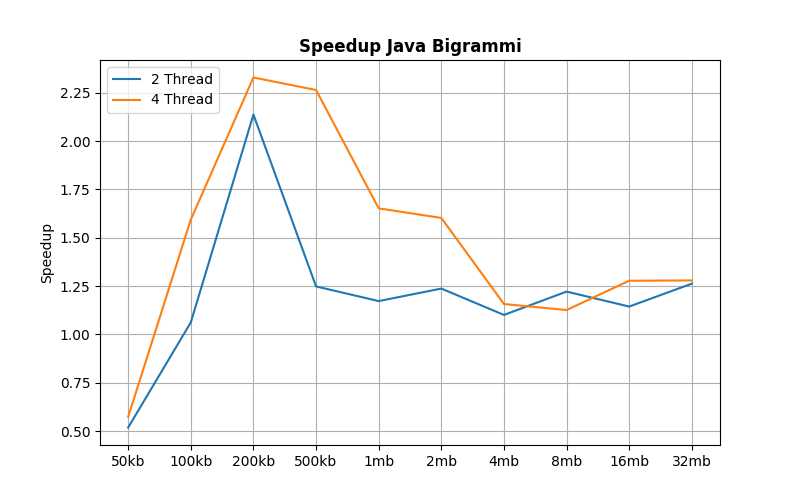
\includegraphics[width=\linewidth]{Plots/speedup_java_bigrammi.png}
\caption{Speedup Bigrammi con Java Thread}
\end{figure}

\begin{figure}[h]
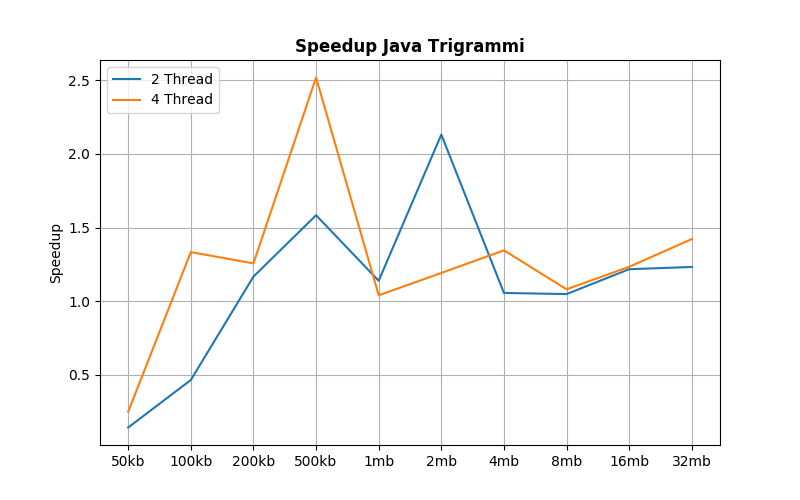
\includegraphics[width=\linewidth]{Plots/speedup_java_trigrammi.png}
\caption{Speedup Trigrammi con Java Thread}
\end{figure}

\subsection{Valutazione dello Speedup con C++ Thread}
Anche in questo caso è stato scelto di utilizzare 2 o 4 thread.
Dunque date le varie dimensioni del file è stato misurato lo \textit{Speedup} al variare delle dimensioni.\newline
Come si può notare dalle immagini, dopo una certa soglia ($\approx$ 16 mb) c'è un aumento significativo dello Speedup.\newline
È ragionevole pensare che aumentando ulteriormente la dimensione del file, si possa ottenere uno Speedup ancora maggiore.

\begin{figure}[h]
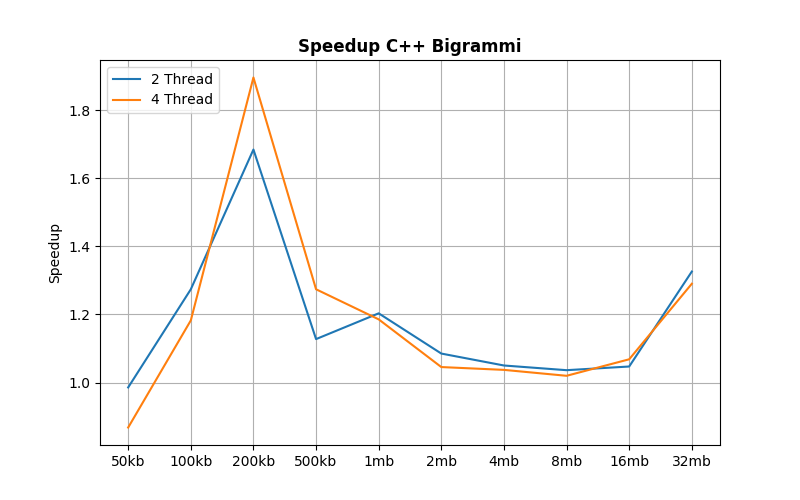
\includegraphics[width=\linewidth]{Plots/speedup_cpp_bigrammi.png}
\caption{Speedup Bigrammi con C++ Thread}
\end{figure}

\begin{figure}[h]
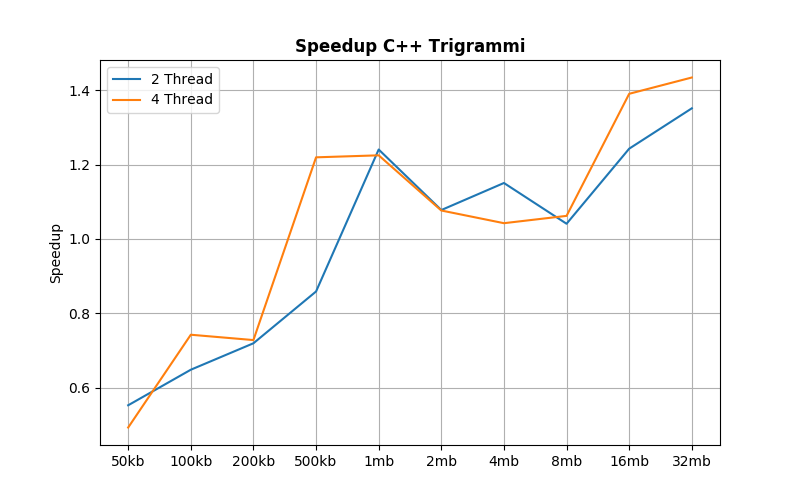
\includegraphics[width=\linewidth]{Plots/speedup_cpp_trigrammi.png}
\caption{Speedup Trigrammi con C++ Thread}
\end{figure}
\newpage

\subsection{Confronto sui Tempi di Esecuzione con Java Thread}
Per avere dei risultati più accurati, è stato eseguito un  confronto anche sui tempi di esecuzione.\newline
Come si può chiaramente notare dai risultati ottenuti, da una certa dimensione in poi ($\approx$ 2 mb) gli approcci paralleli risultano sempre più efficienti rispetto all'approccio sequenziale. Non sono state riscontrare differenze sostanziali tra l'utilizzo di 2 o 4 thread.
\begin{figure}[h]
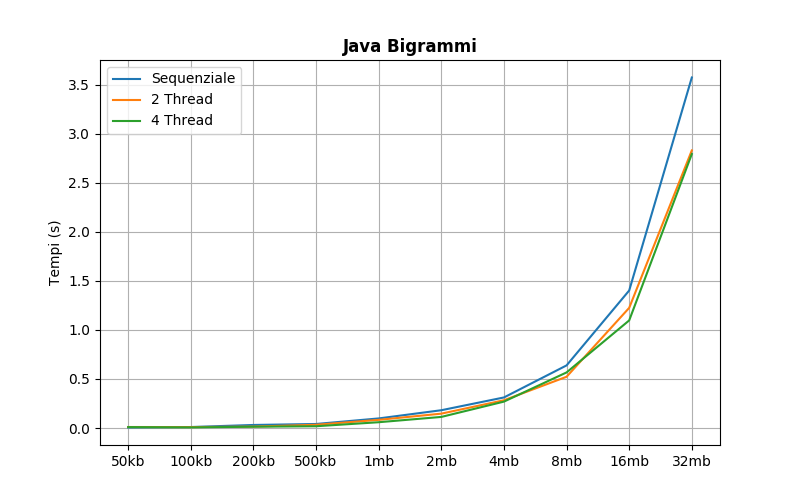
\includegraphics[width=\linewidth]{Plots/tempi_java_bigrammi.png}
\caption{Confronto tempi di esecuzione Bigrammi Java}
\end{figure}

\begin{figure}[h]
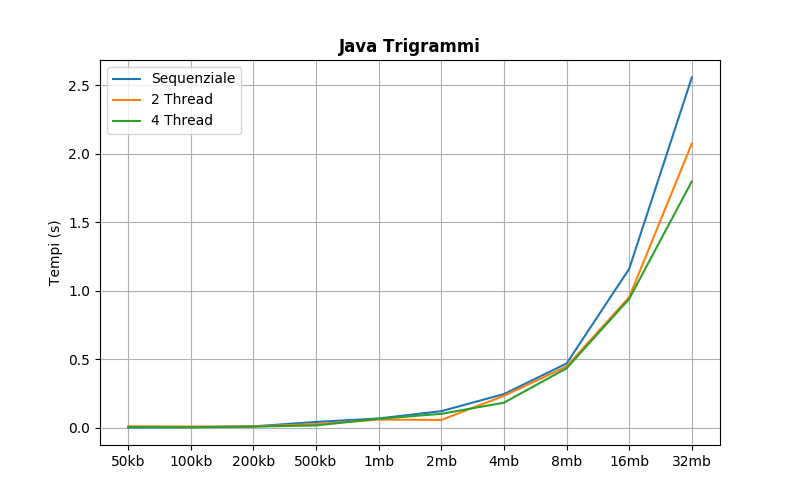
\includegraphics[width=\linewidth]{Plots/tempi_java_trigrammi.png}
\caption{Confronto tempi di esecuzione Trigrammi Java}
\end{figure}
\newpage

\subsection{Confronto sui Tempi di Esecuzione con C++ Thread}
Per avere dei risultati più accurati, è stato eseguito un  confronto anche sui tempi di esecuzione.\newline
Come si può chiaramente notare dai risultati ottenuti, da una certa dimensione in poi ($\approx$ 8 mb) gli approcci paralleli risultano sempre più efficienti rispetto all'approccio sequenziale. Non sono state riscontrare differenze sostanziali tra l'utilizzo di 2 o 4 thread.
\begin{figure}[h]
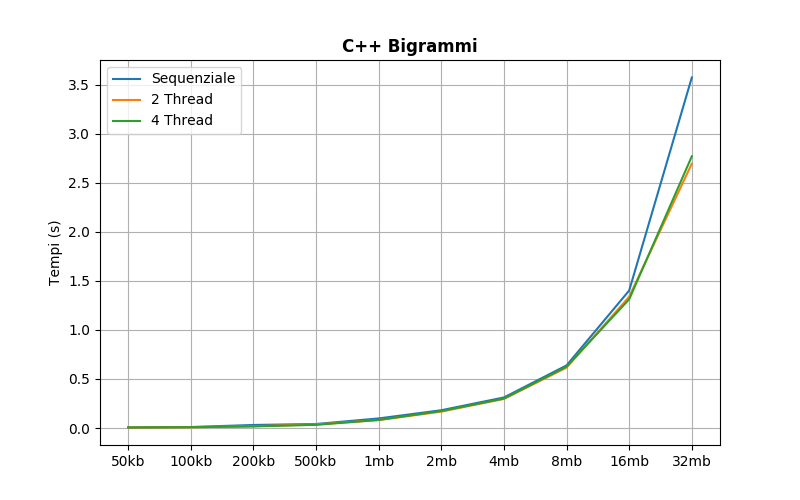
\includegraphics[width=\linewidth]{Plots/tempi_cpp_bigrammi.png}
\caption{Confronto tempi di esecuzione Bigrammi C++}
\end{figure}

\begin{figure}[h]
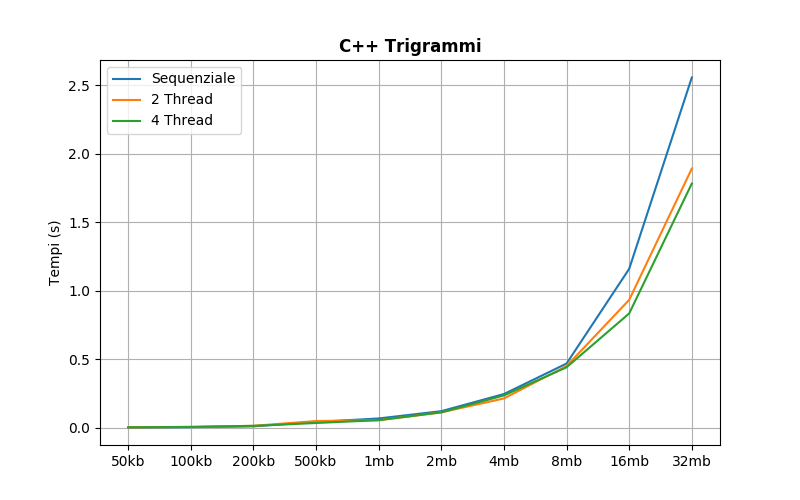
\includegraphics[width=\linewidth]{Plots/tempi_cpp_trigrammi.png}
\caption{Confronto tempi di esecuzione Trigrammi C++}
\end{figure}
\newpage

\section{Conclusione}
Come era possibile aspettarsi per file di grosse dimensioni l'approccio parallelo è sicuramente migliore di quello sequenziale.\newline
In base ai risultati ottenuti si può anche notare che il tempo di esecuzione per la ricerca di bigrammi e trigrammi è leggermente inferiore per i Java Thread rispetto ai C++ Thread.
Considerando anche il fatto che non è stato calcolato il tempo di estrazione di righe e parole, che risulta essere significativamente maggiore (circa 3 volte) con C++ rispetto al Java.

{
\bibliographystyle{unsrt}
\bibliography{bibliografia.bib}
}


\end{document}
